As running example, we consider a grade crossing semaphore and we assume that the designer has identified three simple requirements.
Requirement $\phi_1$ specifies that $red$ lights up  infinitely often ($\LTLglobally\LTLfinally red$), which forces cars to stop when the train approaches the crossing.
Requirement $\phi_2$  states that $green$ lights up infinitely often ($\LTLglobally\LTLfinally green$), which allows the cars to traverse the crossing.
Finally, requirement $\phi_3$ specifies that always, after $red$, $green$ is permanently on ($\LTLglobally (red \LTLimplication \LTLglobally green)$).
Note that $\phi_3$ is wrong (i.e., it does not capture desirable behaviors in the current context). Nevertheless it is used for illustration purposes.

Starting from this specification, suppose that the designer proposes the incompletely specified model of the semaphore shown in Figure~\ref{fig:modelmot}. Each state is associated with the values of the propositions $g$ and $r$ (denoting $green$ and $red$) holding in that state, which specify whether the green and the red lights are on or off in that state.
For example, in state $s_0$ the red light is on ($r=\LTLtrue$) while the green is off ($g=\LTLfalse$).
Instead,  $s_2$ is a state to which the semaphore may be brought, for instance by a manual command. 
The designer still has to choose whether, in this state, the green and red lights should be on or off.
This is indicated by associating the value $?$ to the propositions $g$ and $r$.
The designer might refine the model by setting to either $\LTLtrue$ or $\LTLfalse$ the $g$/$r$ proposition in $s_2$.

%While the behavior in $s_0$ and $s_1$ is fully specified, the designer is uncertain on how the semaphore works in $s_2$.
%More precisely, in the state $s_0$ the semaphore is red while in $s_1$ it is green. 
%The semaphore repeatedly moves from $s_0$ to $s_1$ and vice versa. 
%However, at some point, the semaphore may be manually moved into the state $s_2$.
%This may occur when an anomalous event is detected, such as an accident or an emergency condition.
%At the current development stage state $s_2$ is unspecified.
%Should the $red$, the $green$ light, or both of them be turned on?
%Note that the design of the system behavior in state $s_2$ may also be assigned to a third party company.


%Liveness and safety requirements are among the most interesting and common temporal properties that we might request. 
%For illustration purposes, we would like to make sure that in $M$ $red$ infinitely often lights up ($\phi_1$). On the other hand, we also want to enforce that contradictory messages are not sent out forever: \emph{does it ever happen that eventually permanently red and green are lightened up simultaneously?} ($\phi_2$).
%In addition, we also request a simple liveness property $\phi_3$, ``infinitely often green'', since it is important that the passage is always eventually allowed.

%We are proposing a comprehensive framework that allows the designer to examine these properties satisfiability in $M$. 


\begin{figure}[b]
 \centering
\begin{tikzpicture}[scale=0.33] %[x={10.0pt},y={10.0pt}]

\node [state, initial, initial text={},initial where=above](s_0)
[label={
[align=center,yshift=0.1cm]
%above:
% 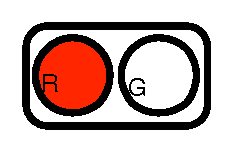
\includegraphics[width=50pt]{images/Red.pdf}
%$\boldsymbol{\overline{green}=T}$\\
$g=\color{black}\bot$\\
$r=\LTLtrue$
}] 
{$s_0$};   


\node[state] (s_1) 
[left=of s_0,
label={
[align=center,yshift=0.1cm]
%above:
% 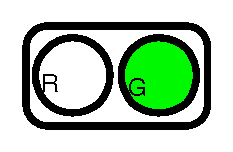
\includegraphics[width=50pt]{images/Green.pdf}
%$\boldsymbol{\overline{green}=F}$\\
$g=\color{black}\LTLtrue$\\
$r=\bot$
}]  
{$s_1$};

\node[state] (s_2) 
[right=of s_0,
label={
[align=center,yshift=0.1cm]
%above:
% 
\includegraphics[width=50pt]{images/Bo.pdf}
%$\boldsymbol{\overline{green}=\bot}$\\
$g=\color{black}?$\\
$r=?$
}]  
{$s_2$};


\path[->]      
(s_0) edge [bend left] node [above]{} (s_1) 
(s_1) edge [bend left] node [above]{} (s_0)
(s_0) edge [bend left] node [above]{} (s_2)
(s_2) edge [bend left] node [above]{} (s_0);   

\end{tikzpicture}
\caption{System model $M$}
\label{fig:modelmot}
\end{figure}


Regardless of the temporary incompleteness, the designer wants to evaluate the satisfaction of the properties of  interest. 
By model checking, it is possible to verify that the model does not contain any behavior that violates or possibly violates $\phi_1$. 
However, the result does not provide any information on why $\phi_1$ is satisfied.
Instead, a model checker equipped with a deductive verification framework would reveal that the system enters infinitely often state $s_0$, in which the red light is turned on, thus explaining why property $\phi_1$ is satisfied.

Let us now consider property $\phi_2$, which possibly holds.
The model checking algorithm returns a \emph{possible} counterexample: by turning off the green light in state $s_2$, the system may infinitely loop over $s_0$ and $s_2$ without $g$ ever being true. 
However, the search of a \emph{definitive} counterexample has failed.
The deductive verification framework would explain to the designer why this search failed.
As a matter of fact, if a counterexample is present, it must be present in any possible completion  of the model, i.e., for any possible assignment to the light in the state $s_2$.
But, let us consider a possible refinement of the incomplete state $s_2$ where the green light is on.
Since the green light is on in $s_1$ ($s_2$), it is possible to deduce that the light is eventually green in state $s_1$ ($s_2$).
Since it is allowed to loop over states $s_0$, $s_1$ and $s_2$, it is possible to deduce that ``always eventually green" is true in $s_0$, $s_1$ and $s_2$.
Thus, $\phi_2$ is satisfied in $s_0$, the initial state.
In conclusion, when the model checker returns maybe, it outputs a possible counterexample for a possible refinement of the incomplete states. 
In addition, the deductive verification framework would explain that the search of a definitive counterexample has failed in the case in which the green light is on in $s_2$.
This provides a useful insight to the designer, explaining that, by setting $g$ to $\LTLtrue$ in $s_2$, one obtains a model satisfying $\phi_2$ while, in the opposite case, $\phi_2$ is violated.


Finally, when property $\phi_3$ is considered, the model checking algorithm returns a definitive counterexample since $\phi_3$ is not satisfied, regardless of further refinements of $s_2$. Indeed, there exists an infinite run among states $s_0$ and $s_1$ in which a red light is not followed by a permanently green light. Indeed, the requirement that the designer probably meant to specify is $\LTLglobally (red \LTLimplication \LTLnext green)$.



%
%The model checker returns an ``unknown'' answer because if, in a future implementation, the semaphore is green in $s_2$, then the property holds. On the contrary, should not the green light be configured in $s_2$, the property would be violated.
%
%What our proposed approach offers is the ability to jointly analyze both potentially bad designs and potentially good designs.
%Especially in those cases where the model checker answer is ``unknown'', the designer is provided with information that can reveal itself fundamental to complete the current design. Namely: he/she obtains a counterexample that shows one violating behavior along with a proof that justifies why the current implementation of the model does not violate the property.
%The counterexample returned corresponds to the scenario in which the system infinitely loops over states $s_0$ and $s_2$.
%The provided proof explains  to the designer \emph{why} the search of a violating behavior has failed.
%This procedure considers a version of $M$ in which the $?$ values are substituted with $\LTLtrue$.
%It first identifies a set of axioms that specify why the search fails in some states of the model.
%By using a set of deductive verification rules it shows how these axioms imply the overall satisfaction of $\phi_3$.
%In this example, we first state what axiomatically holds in the states $s_1$ and $s_2$, which are the peripheral areas of the model.
%Since $s_1$ and $s_2$ are successors of $s_0$ we can inductively deduce what is satisfied in $s_0$. The final result, is reached by conjucting all the conclusiones gathered on the single model states.
%

%%%%
